\chapter{Subdivision Example} \label{ch:test}

\lipsum[1-2]


\section{One fine Section} \label{sec:fine}

\lipsum[1]

\subsection{Subsection}

\subsubsection{Subsubsection}

\paragraph{Paragraph} \lipsum[2]



\chapter{Tables Example} \label{ch:tab}

% standard issue
\begin{maketable}
	\caption{CHANGE THIS}
	\label{tab:CHANGE_THIS}
	\begin{maketablebody}{wide}{ X  l  l  l  l }\toprule %narrow, normal, wide or full (or number between 0 and 1)
		\textbf{Setup} & \textbf{\# Stiffeners} &
		\textbf{Stiffener pitch ($mm$)} &
		\textbf{$\tau_{cr}$ ($MPa$)} & \textbf{$\tau$ ($MPa$)}\\\midrule
		Set-up 1 & 5 & 331.2 & 3.04 & 10.42 \\
		Set-up 2 & 6 & 265.0 & 5.28 & 10.42\\
		Set-up 3 & 7 & 220.8 & 8.36 & 10.42\\
		Set-up 4 & 8 & 189.2 &12.29 & 10.42\\
		Set-up 5 & 9 & 165.6 &16.89 & 10.42\\
		\bottomrule
	\end{maketablebody}
\end{maketable}

% 90° rotated
\newpage
\begin{centering}

    \rotatebox{90}
    {\begin{minipage}{0.9\textheight} % you can play with this value, depending on whether there is a section title on the same page
    	\centering
    	\captionsetup{type=table,width=0.55\textheight} % keep this value fix please
    	\captionof{table}{CHANGE THIS}
    	\label{fig:CHANGE_THIS}
    	\begin{maketablebody}{full}{ X  X  X X X  X }\toprule %narrow, normal, wide or full (or number between 0 and 1)
    		\textbf{Mission} & \textbf{Objective} & \textbf{Element functions} \\\midrule
    		ExoMars TGO  & 9 & 165.6 \\
    		\bottomrule
    	\end{maketablebody}
    \end{minipage}}

\end{centering}

% segmented table
\begin{maketable}
	\caption{CHANGE THIS}
	\label{tab:CHANGE_THIS}
	\begin{maketablebody}{wide}{ X  l  l  l  l }\toprule %narrow, normal, wide or full (or number between 0 and 1)
		\textbf{Setup} & \textbf{\# Stiffeners} &
		\textbf{Stiffener pitch ($mm$)} &
		\textbf{$\tau_{cr}$ ($MPa$)} & \textbf{$\tau$ ($MPa$)}\\\midrule
		Set-up 1 & 5 & 331.2 & 3.04 & 10.42 \\
		Set-up 2 & 6 & 265.0 & 5.28 & \makecell[tl]{Some\\ more \\ stuff}\\
		Set-up 3 & 7 & 220.8 & 8.36 & 10.42\\
		Set-up 4 & 8 & 189.2 &12.29 & 10.42\\
		Set-up 5 & 9 & 165.6 &16.89 & 10.42\\
		\bottomrule
	\end{maketablebody}
\end{maketable}








\clearpage
\chapter{Figures Example} \label{ch:fig}

% standard issue
\begin{makefigure}
    \insertpicture{wide}{ADCS.png}  % narrow, normal or wide (or number between 0 and 1)
    \caption{CHANGE THIS}
    \label{fig:CHANGETHIS}
\end{makefigure}

% subfigures
\begin{makefigure}

	\begin{makesubfigure}{0.5} % these values must add up to 1 (or slightly below). 
		\insertpicture{wide}{ADCS.png} % narrow, normal or wide
		\caption{CHANGE THIS}
		\label{fig:CHANGE_THIS} % do not forget the "%" sign below, it is actually important
	\end{makesubfigure}% 
	\begin{makesubfigure}{0.5}
		\insertpicture{wide}{ADCS.png}
		\caption{CHANGE THIS}
		\label{fig:CHANGE_THIS}
	\end{makesubfigure}
	
    \caption{Schematic overview of the strain gauge locations on top and bottom panel.}
    \label{fig:CHANGE_THIS}
\end{makefigure}

% rotated
\begin{centering}
    \rotatebox{90}
    {\begin{minipage}{0.7\textheight} % you can play with this value, depending on whether there is a section title on the same page
        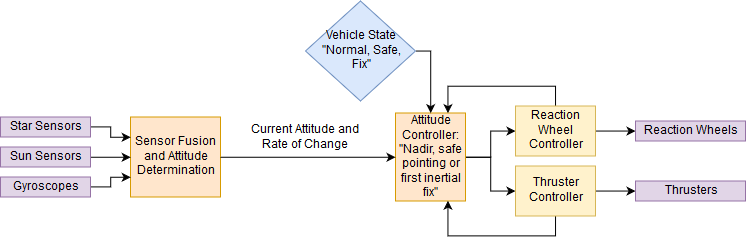
\includegraphics[width=0.7\textheight]{ADCS.png}% this value must match the one above
    	\captionsetup{type=figure,width=0.55\textheight} % keep this value fix please
    	\captionof{figure}{CHANGE THIS}
    	\label{fig:CHANGE_THIS}
    \end{minipage}}
\end{centering}




\chapter{Equations Examples}

%single line:

\begin{align} \label{eq:CHANGETHIS}
    \begin{split}
        \sigma_x = \frac{E^s(\epsilon_x+\nu\epsilon_y)}{1-\nu^2}
    \end{split}
\end{align}


%multiple lines, aligned at the "&", one separate label for each

\begin{align} \label{eq:CHANGETHIS}
    \sigma_x &= \frac{E^s(\epsilon_x+\nu\epsilon_y)}{1-\nu^2} \\
    \sigma_y &= \frac{E^s(\epsilon_y+\nu\epsilon_x)}{1-\nu^2}
\end{align}



%multiple lines, aligned at the "&", only one label

\begin{align} \label{eq:CHANGETHIS}
    \begin{split}
        \sigma_x &= \frac{E^s(\epsilon_x+\nu\epsilon_y)}{1-\nu^2} \\
        \sigma_y &= \frac{E^s(\epsilon_y+\nu\epsilon_x)}{1-\nu^2}
    \end{split}
\end{align}


%side by side:

\begin{align} \label{eq:CHANGETHIS}
    \begin{split}
        \sigma_x = \frac{E^s(\epsilon_x+\nu\epsilon_y)}{1-\nu^2} \quad \quad
        \sigma_y = \frac{E^s(\epsilon_y+\nu\epsilon_x)}{1-\nu^2}
    \end{split}
\end{align}


%matrix stuff
\begin{align}
    \begin{split}
    \begin{pmatrix}  F_x & 1\\ 0&2\\ F_z&3\end{pmatrix}
    \end{split}
\end{align}



\chapter{Citing Example}

\section{Writing the bib file}

Write them into the file \texttt{aa\_lists/bibliography.bib} (there are example inside this file). General Remarks:

\begin{itemize}
    \item Always search for an already existing entry of the thing you want to reference first
    \item Also, make the identifier of the entry (the string that you use to cite it in-text) meaningful, maybe more meaningful than things like "nasaa" or the like.
    \item If you do not know a field (like year), just leave the entire line out, do \emph{not} use year="-" or author="unknown" or the like.
    \item End all lines BUT THE LAST LINE of an entry with a comma "," 
\end{itemize}

Author formatting: The BibLaTeX package is relatively smart and configurable in terms of these things. Always use all the full names and titles of all authors in their natural order, separated by "and":
\begin{itemize}
    \item "John D. Anderson and Prof. Jacco Hoekstra and Dr. Lonnie Smith and Jimi Hendrix and James Brown and Bill Withers"
\end{itemize}

Company formatting: If you only know the company name and no authors, put it in curly brackets like this: 
\begin{itemize}
    \item "{The Hammond Organ Company}"
\end{itemize}

Avoid the @misc category. For example, if you find a pdf online that is actually a book, use the @book class.



\section{Using citations in-text}

After a sentence (AND \emph{AFTER} THE FULL STOP "."), just do this. \autocite{hendrix70}

Use \texttt{textcite} if you embed the citation into the sentence for getting something like : "Excessive use of drugs and alcohol frequently lead to artists death as described in \textcite{hendrix70}"

Whenever applicable, use page numbers of section number like this: \autocite[p.42-70]{hendrix70} or \autocite[Section "3rd Stone From The Sun"]{hendrix70}





\chapter{Cross Ref Example}

Use \texttt{label} formats like this: \label{ch:CrossRef}. You can use the following prefixs:
\begin{itemize}
    \item ch: chapter
    \item sec: sections (and subsections)
    \item tab: table
    \item fig: figure
    \item eq: equation
\end{itemize}

Manually put things like "section" or "sections" (and so on) in front of "chapter \ref{sch:CrossRef}", I have not set up LaTeX to do stuff like that itself.

Do not use "Subsection" in the text (it is not really a word), use "Section" regardless of its level in the text.




\chapter{Fancy Boxes}

\begin{FancyBox}{Introduction}
    Inconclusive yes.
\end{FancyBox}

\begin{SideBar}{Question:}
    Which bear is best? \lipsum[1]
\end{SideBar}


